This chapter investigates magneto-plasmonics, the ability to perturb a plasmonic response with magnetic fields, in gold nanoparticles. Magneto-plasmonics is generally associated with ferromagnetic-plasmonic materials because such optical-derived responses from nonmagnetic materials alone are considered weak, however, this chapter shows the measurable magneto-optical responses in gold nanoparticles. This chapter shows that there exists a transition between linear and nonlinear magneto-optical behaviors in gold nanocolloids that is observable at ultra-low illumination intensities and direct-current magnetic fields. The response is attributed to polarization-dependent nonzero-time-averaged plasmonic loops, vortex power flows, and nanoparticle magnetization. This chapter identifies significant mechanical effects that arise via magnetic-dipole interactions, exhibited via changes in the transmission spectra.

\section{Introduction}
The plasmonic resonances of noble metal nanostructures manifest in the visible spectral range and have a fundamental role in shaping the optical properties of materials [\cite{Link,Cortie}]. At such resonances the electromagnetic fields are concentrated around sub-wavelength structures producing high local field enhancements, which has been the study of many investigations [\cite{Barnes,Kelly03,Ozbay}]. Since the resonances are highly dependent on the refractive index of the material, as well as the surrounding medium, methods that modify a materials refractive index \textit{i.e.,} electro-optically [\cite{Dicken,Chyou}] or thermally [\cite{Nikolajsen}], are realised by a shift in the plasmonic resonance. An external magnetic field can also modulate a material's optical properties if the material exhibits magneto-optical (MO) behaviour [\cite{Temnov,Gonzalez,Deng}]. The concurrent application of a magnetic field is associated with additional phenomena such as increased Faraday rotation [\cite{Du}], MO enhancement of localized and propagating surface plasmons [\cite{Sepulveda,Torrado}], or introduction of new magnetic modes [\cite{Pineider,Tang,FanSci}]. Observations of these MO phenomena, however, are generally small unless the plasmonic material is mated with a ferromagnet. Another class of MO responses involves non-oscillating, DC, magnetic modes. Such modes are achieved in non-magnetic media via the polarization-dependent inverse Faraday effect [\cite{Hertel}] though this DC or low frequency MO response is claimed to be too small to observe at room temperature and at low intensities due to thermal fluctuations [\cite{Gu}] (the effect is observed with high intensity lasers, $>$370 MW/cm$^2$ [\cite{Raja}]). Anomalously-large photo-induced magnetic responses are observed in non-ferromagnetic metal nanocolloids [\cite{Singh}], however the origin of the effect is unexplained. This chapter identifies and analyses the threshold transition between linear and nonlinear effects, which is attributed to a mechanical response of the nanocolloid.

This chapter demonstrates that nonzero time-averaged vortex currents on nanostructures enable the magnetization of non-magnetic materials and that such DC MO plasmonic responses are observable with broadband light illumination intensities less than 1 W/cm$^2$. Moreover, there exists a nonlinear MO response that is explained by the theoretical model of \cite{Hertel} when applied to nanostructures [\cite{Singh, Brandao, Bliokh}]. This coupling between incident and scattered fields yields nonzero time-averaged azimuthal vortex power flows that differ distinctly in character from the polar-coordinate whirlpool flows investigated in other work [\cite{Boriskina,Bashevoy}]. The vortex power flows associated with azimuthal currents that result in the formation of DC magnetic dipoles is quantified. More importantly, it is demonstrated that such dipoles are non-negligible and external magnetic fields influence the nanocolloidal optical properties. Experimentally, the response is observed in the extinction spectra of aqueous 80-nm gold nanospheres when illuminated with circularly-polarized light and DC magnetic fields, in which changes occur on minute time-scales. The retarded response is attributed to magnetic-dipole interactions and the mechanical movement and settling of asymmetrical nanoparticles and nanoclusters. The formation of realizable DC magnetic dipoles and the associated mechanical effects are verified in numerical simulations.

Both linear and nonlinear plasmon phenomena lead to MO responses. Linear characteristics associated with volume charge densities are distinct from nonlinear characteristics associated with surface charges, which dominate the MO response above low-threshold magnetic fields. The linear dynamics are described by a conventional Hall-effect Drude model [\cite{Mulvaney}], which provides a magnetic-field dependent refractive index via the Lorentz force. In contrast, the nonlinear dynamics are identified with the inverse Faraday effect, which yields a nonlinear current density proportional to the incident electric field intensity [\cite{Hertel}]. It is fundamental to the analysis that while there is no net current i.e., $\langle\vec{j_x}\rangle= \langle\vec{j_y}\rangle= \langle\vec{j_z}\rangle=0$, non-zero time-averaged current loops exist such that $\langle\vec{j_{\phi}}\rangle \neq 0$. This existence of nonzero $\langle\vec{j_{\phi}}\rangle$ forms the basis of the nonlinear DC MO response.
\section{Linear dynamics}
\subsection{Addition of magnetic fields to equations of motion}

The linear dynamics of the volume charge density, within the quasi-static limit [\cite{MaierBook}], are governed by the equations of motion with the Lorentz force: $m^*\frac{d^2\vec{r}}{dt^2}+m^*\gamma\frac{d\vec{r}}{dt} = q\vec{E} + q(\frac{d\vec{r}}{dt}\times\vec{B})_r-k\vec{r}$, where $\vec{r}$ denotes the spatial coordinate, $m^*$ is the effective mass of the electron, $\gamma$ is the decay rate, $q$ is the charge of an electron, and $k$ is the force constant associated with the restoring force. The electric field propagates in the $\hat{z}$ direction with time-harmonic circular-polarization of angular frequency $\omega$ and amplitude $E_0$, $\vec{E_{\pm}}=E_0 e^{-i\omega t}(\hat{x}\pm i\hat{y})/\sqrt{2}$, where $+(-)i\hat{y}$ represents a right(left)-handed circular-polarized wave or RHCP(LHCP). When an externally-applied DC magnetic field is aligned with the direction of the electric-field propagation, $\vec{B}=B_0\hat{z}$, the equations of motion yield a dielectric function in the form of a gyrotropic tensor: $\epsilon=1+ \omega_p^2\Bigl(\begin{smallmatrix} \alpha& -\beta &0\\ \beta &\alpha&0\\0&0&\zeta\end{smallmatrix}\Bigr)$, in which $\alpha=\frac{\omega_0^2-\omega^2-i\gamma\omega}{(\omega_0^2-\omega^2-i\gamma\omega)^2+(\omega\omega_c)^2}$, $\beta=\frac{i\omega\omega_c}{(\omega_0^2-\omega^2-i\gamma\omega)^2+(\omega\omega_c)^2}$, and $\zeta=\frac{1}{\omega_0^2-\omega^2-i\gamma\omega}$, where $\omega_c=qB_0/m^*$ is the cyclotron frequency, $\omega_p$ is the plasma frequency such that $\omega_p^2 = \eta q^2/m^*\epsilon_0$, $\omega_0$ is the frequency associated with a harmonic restorative force, and $\eta$ is the electron density.  The Lorentz force is largest when the DC magnetic field is parallel to the propagation of light [\cite{Sepulveda}].
\\
\begin{figure}[t]
\centering
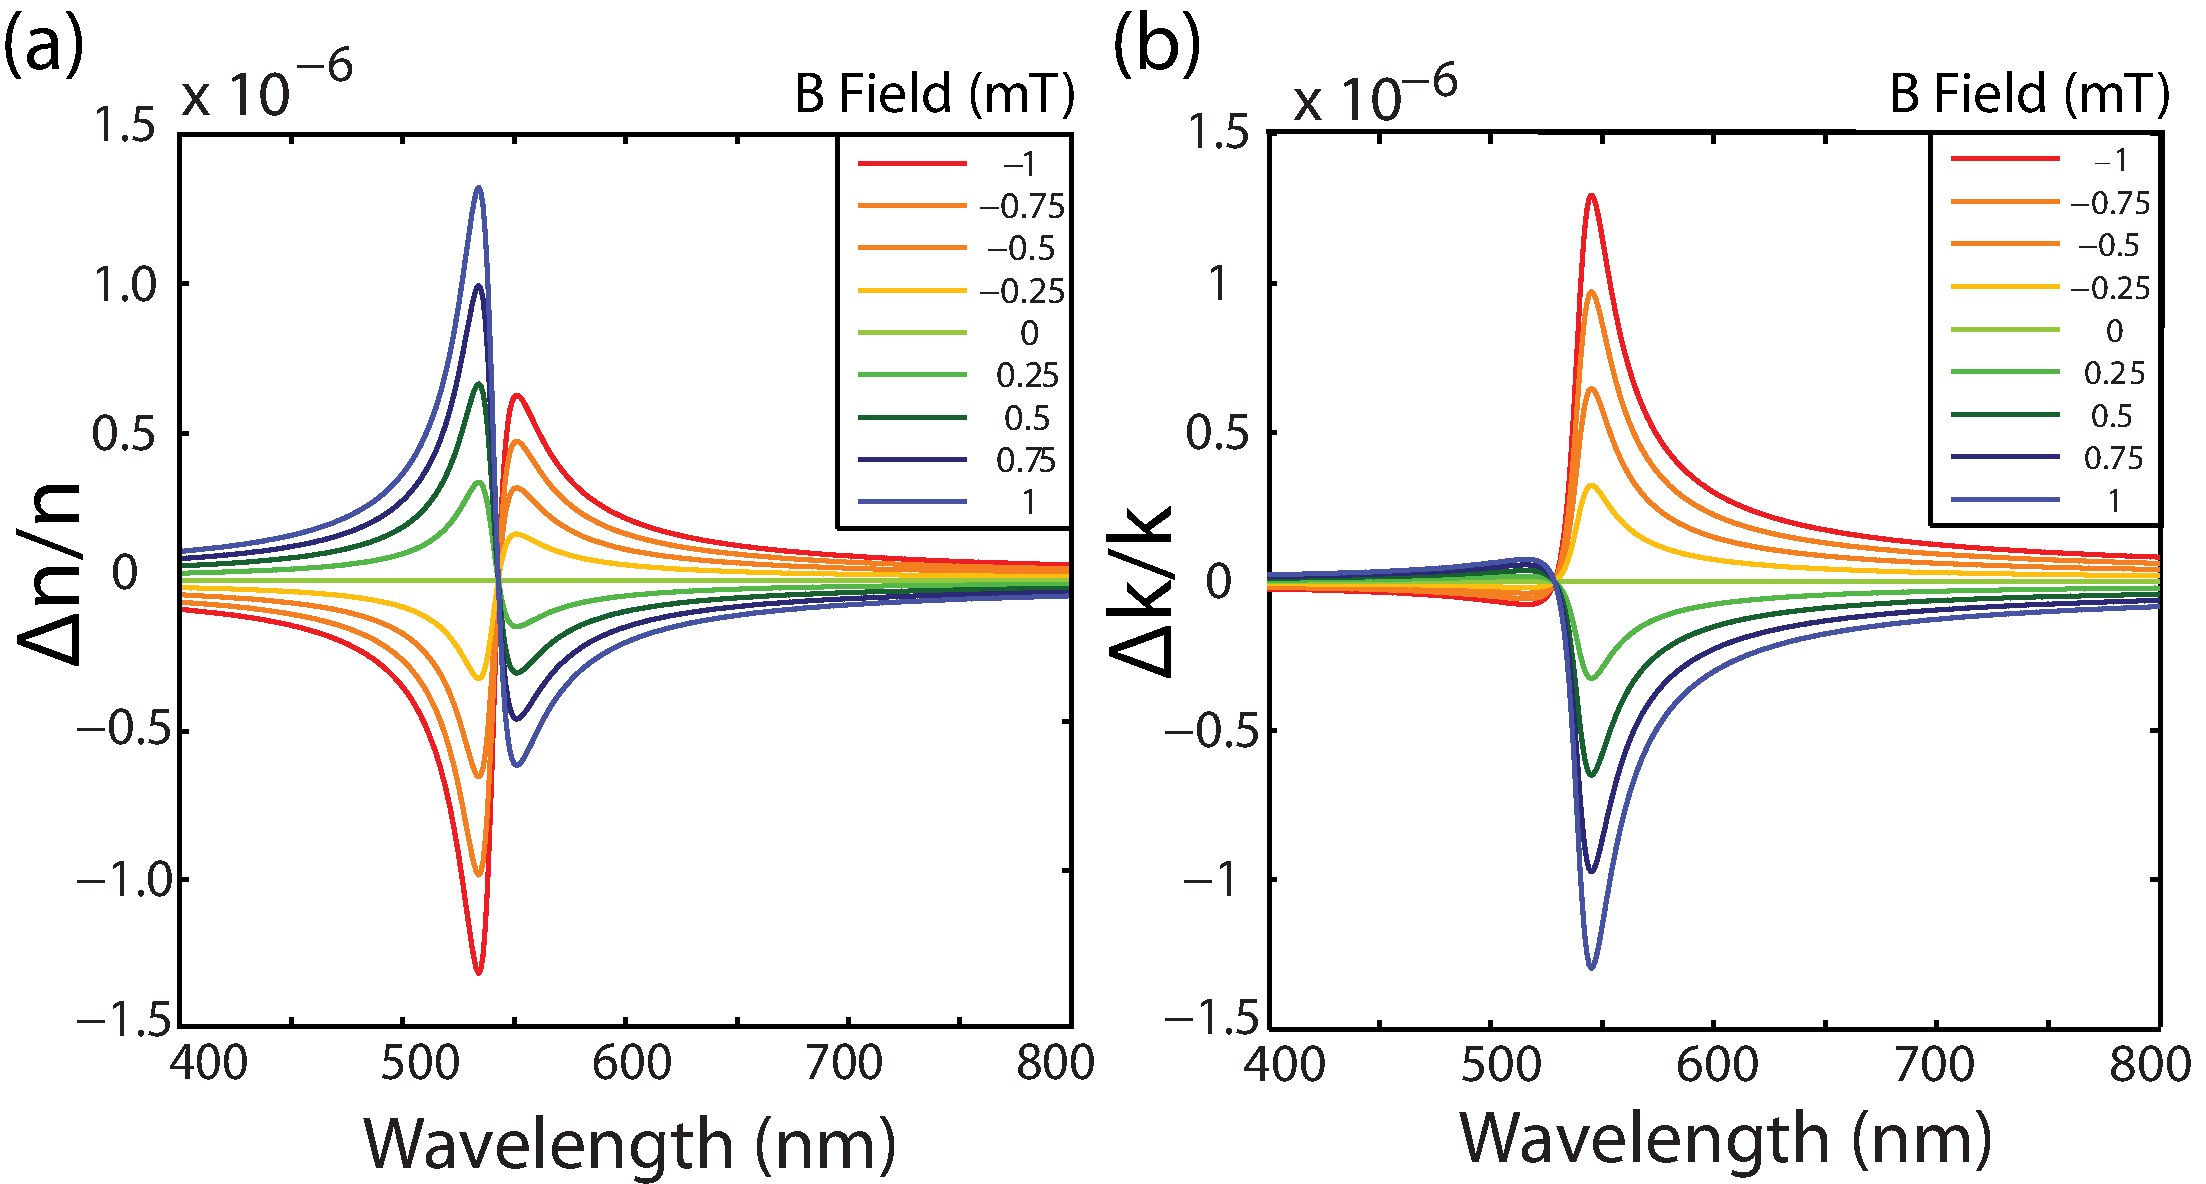
\includegraphics[width=\textwidth]{dnk_mT.pdf}
\caption{Relative MO shift of bulk gold when external fields are varied. (a) Real and (b) imaginary parts of the refractive index as a function of wavelength under illumination of 1 W/cm$^2$ RHCP when magnetic fields are varied.}
\label{fig:1}
\end{figure}

As can be seen in Fig.~\ref{fig:1}, around the plasmon resonance (540 nm) there are significant shifts in the real and imaginary parts of the refractive index. This MO model explains the response from small magnetic-field perturbations, however is insufficient to explain the changes in optical properties at higher applied magnetic fields [\cite{Singh}]. The MO response of noble metals (calculated with linear dynamics) is significantly smaller compared to that which occurs with ferromagnets in part because the difference between the cyclotron and plasma frequencies is orders of magnitude apart [\cite{Schnatterly}]. Moreover, the MO response depends on other factors such as the exchange interaction, specific band structure and spin-orbit coupling that allow ferromagnetic materials to have a greater MO response than noble metals [\cite{Armelles2}].  
\section{Nonlinear dynamics}
\subsection{Nonlinear current density}
In departure from prior investigations of MO effects on nanostructures, an analytical expression derived from the continuity equation [\cite{Hertel}] describes a time-averaged solenoidal magnetization current density:
\begin{equation}
\langle \vec{j_m} \rangle = \frac{i}{4q\langle \eta\rangle \omega}\nabla \times\big(\sigma_0^*\vec{E}^*\times\sigma_0\vec{E}\big),
\label{jm_eqn}
\end{equation}
where $\langle \eta\rangle$ is the time-averaged electron density, $\sigma_0$ is the specific conductivity of gold, and $\vec{E}$ is the total electric field at the surface. As seen in Eq.~\ref{jm_eqn} $\langle\vec{j_m}\rangle$ is polarization-dependent in its direction and magnitude. For a circularly-polarized $\vec{E}$ the term $\vec{E_{\pm}}\times\vec{E_{\pm}^*}$ becomes $\pm i |\vec{E_0}|^2\hat{z}$ and for a linearly-polarized field this term is zero. Note that $\langle\vec{j_m}\rangle$ scales inversely with $\langle \eta\rangle$, which may explain MO effects in non-metallic nanostructures [\cite{Kuznetsov}] and also scales with the intensity, in contrast to linear currents which scale with the electric field ($\vec{j}=\sigma_0\vec{E}$). 
\subsection{Nonlinear magnetization}
In this study of nanospheres, the time-averaged nonlinear current density is significant only in the azimuthal direction, $\hat{\phi}$, $\langle\vec{j_{m,r}}\rangle=0$, $\langle\vec{j_{m,\theta}}\rangle\ll \langle\vec{j_{m,\phi}}\rangle$. Although linear time-harmonic azimuthal currents exist, the current direction reverses every 1/2 cycle and time-average to zero. Since the nonlinear surface currents produce an anisotropic field-dependent perturbation to the specific conductivity, it is reasonable to employ a formalism similar to that used for the nonlinear polarization with the nonlinear current density as $\vec{j_p}(\vec{E}) = \vec{j^{(1)}_p}(\vec{E}) + \vec{j^{(2)}_p}(\vec{E},\vec{E}) + ... = \sigma_{p,r}^{(1)}E_q+\sigma_{p,r,s}^{(2)}E_rE_s+...$, where $\sigma^{(1)}_{p,r}$ is the specific conductivity in isotropic media. 
Using Eq.~\ref{jm_eqn} and Levi-Cevita notation $\sigma_{p,r,s}^{(2)}$ can be written as a third-rank tensor in the form:
\begin{equation}
\sigma_{p,r,s}^{(2)} = \frac{i|\sigma_0|^2}{4q\langle\eta\rangle\omega}\frac{\epsilon_{p,r,s} \hat{\partial_r}\epsilon_{s,t,u}E_t^*E_u}{E_{r}E_{s}}.
\label{DelSig}
\end{equation}
A relation for the induced magnetization can also be obtained using $\vec{j_m} = \nabla\times\vec{M}$, such that:
\begin{equation}
\vec{M_p} = \frac{i|\sigma_0|^2}{4q\langle\eta\rangle\omega}\epsilon_{p,r,s} E_{r}^*E_{s}
\end{equation}
\begin{figure}[b!]
\centering
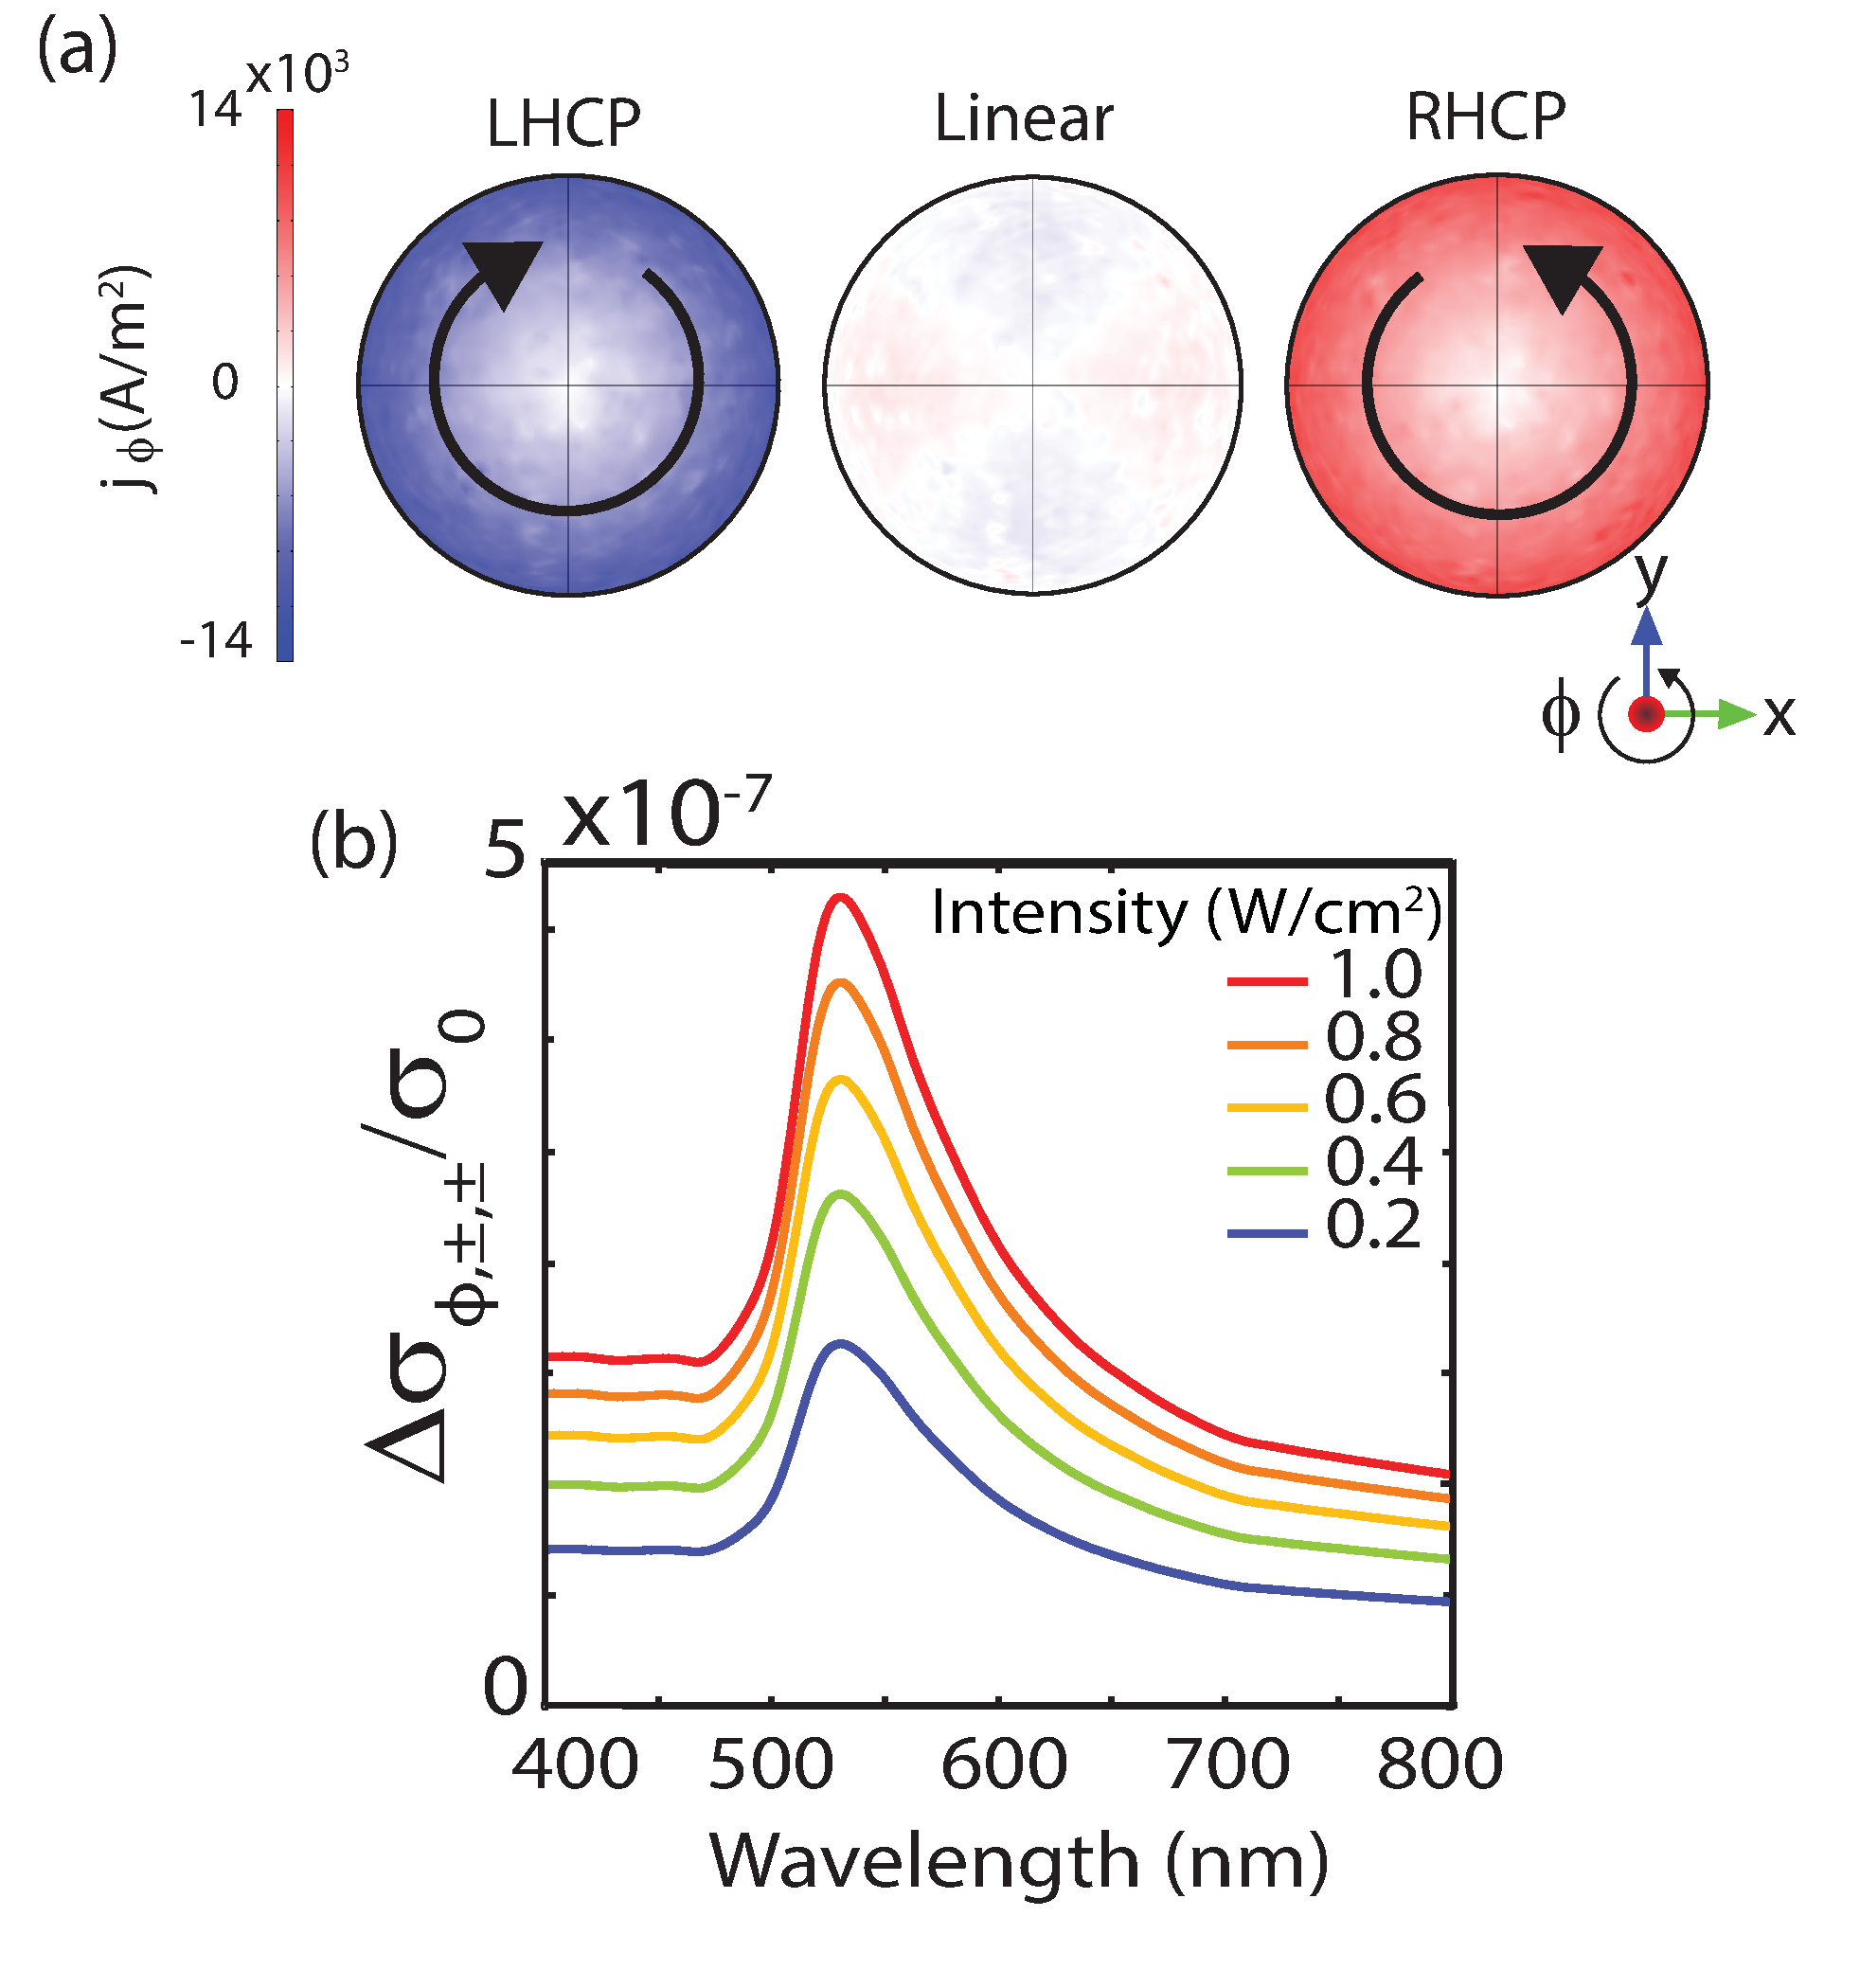
\includegraphics[width=0.95\textwidth]{SigandJPhi8}
\caption{(a) Surface plots of the nonlinear current density of an aqueous 80-nm gold nanosphere when illuminated by LHCP, linearly-polarized and RHCP light in the $\hat{z}$ direction at the plasmon resonance, 540 nm, at 1 W/cm$^2$. (b) Volume-averaged relative change in azimuthal component of the conductivity as a function of wavelength when illumination intensity is varied for RHCP or LHCP.}
\label{fig:2}
\end{figure}
\section{Numerical predictions}
\subsection{Finite-element simulation results}
\indent Numerical, finite-element simulations illustrate the strong polarization dependence of the nonlinear current density that the theoretical analyses predict. As seen in Fig.~\ref{fig:2}(a) the induced nonlinear current density, $\langle\vec{j_{m,\phi}}\rangle$, is calculated for an aqueous 80-nm gold nanosphere illuminated in the $\hat{z}$ direction with different polarizations. To simplify the notation of the nonlinear conductivity response only the first subscript of $\sigma^{(2)}$ that denotes the direction of the anisotropic change. It can be shown that $\sigma^{(2)}$ is nonzero only for curvilinear coordinates such as $\phi$ or $\theta$ in spherical coordinates. The numerical calculations illustrate that $\sigma^{(2)}_{\phi}$ is negligible for incident linear polarization, and RHCP and LHCP yield the greatest $\sigma^{(2)}_{\phi}$ with equal direction and magnitude; as illustrated in Fig.~\ref{fig:2}(b), as the light intensity increases, the conductivity of the nanoparticle also increases uniformly across wavelengths for both RHCP and LHCP. Since both the azimuthal currents ($\propto \nabla\times\vec{E}^*\times\vec{E}$) and the electric-field components ($\vec{E}_\phi$) reverse direction with polarization handedness, by symmetry, the relative changes in the conductivity tensor are identical for both RHCP and LHCP. 

\section{Experimental observation}
\subsection{Observation of transition from linear to nonlinear dynamics}
\begin{figure}[p]
\centering
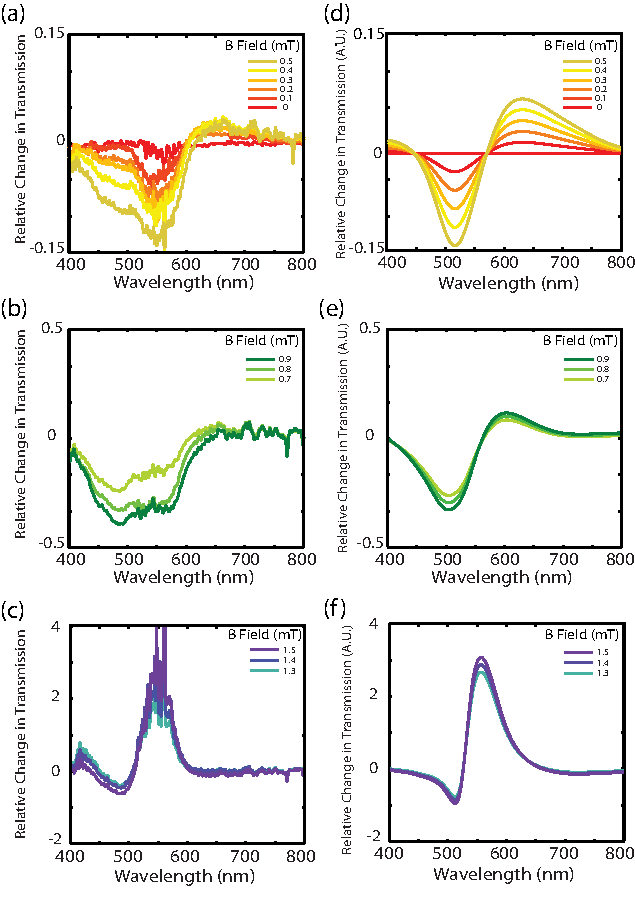
\includegraphics[height=0.95\textheight]{ExExpB11.pdf}
\caption{(Continued on the following page.)}
\label{Exp}
\end{figure}
\addtocounter{figure}{-1}
\begin{figure} [t!]
  \caption{(Previous page.) Normalized MO changes in transmission for aqueous gold nanocolloid at (a) low magnetic fields (b) intermediate magnetic fields and (c) higher magnetic fields. Theoretical MO change in transmission of aqueous 80-nm gold nanospheres in the (d) linear and (f) nonlinear analyses. Theoretical MO changes that combine the linear and nonlinear analyses are shown in (e) for intermediate magnetic fields. In all plots the illumination is 1 W/cm$^2$ and RHCP.}%missing
\end{figure}

\indent Experimental data of relative MO changes in transmission spectra are illustrated in Fig.~\ref{Exp}, alongside analytical results. The experiments were performed with samples of 0.05 mg/mL 80-nm poly-vinyl pyrolidone(PVP)-capped gold nanoparticles dispersed in aqueous solution (2.5$\times 10^{-6}$ fill factor). A solar simulator, polymer thin-film linear polarizer, and 400-800 nm achromatic quarter-wave plate produce RHCP white light, and a Helmholtz coil generates a uniform magnetic field in the direction of light propagation around the sample. A CCD spectrometer that captures the extinction spectra is placed behind a 0.5-cm optical path length cuvette containing samples.
\\\indent The dominant response is dependent on the illuminating light polarization at low magnetic fields and is polarization-independent in the presence of higher magnetic fields; a threshold behaviour exists. Experimentally, a magnetic field of 0.9 mT is associated as the bound between the linear (polarization-dependent) and nonlinear (polarization-independent) dynamics. The experimental data [Fig.~\ref{Exp}(a-c)] shows relative transmission data for RHCP and positive magnetic fields. Below the threshold, differences between the handedness of the polarizations are observed; the MO response is approximately equal and opposite in magnitude. Above, the transmission is similar for both RHCP and LHCP. 
\\\indent The experimental data agrees with analytical theory when the changes of the refractive index [Fig.~\ref{fig:1}] and conductivity [Fig.~\ref{fig:2}(b)] are incorporated to Mie theory [\cite{Mie}] and the corresponding relative changes in extinction spectra are computed. These calculated linear and nonlinear MO responses are shown separately in Fig.~\ref{Exp}(d) and Fig.~\ref{Exp}(f) respectively, and both linear and nonlinear MO responses are incorporated to analyse the total response at intermediate fields near the threshold [Fig.~\ref{Exp}(e)]. The relative change in the nonlinear MO response has been scaled to reflect the experimental behaviour. The nonlinear response is modelled as a function of the external magnetic field, which tunes the strength of the coupling that causes the MO response. The threshold behaviour observed experimentally is expected to occur when the theoretical linear and nonlinear effects are comparable. Moreover, this theoretical model provides excellent quantitative agreement; in this analysis of a single nanosphere the changes in the refractive index and conductivity via the linear and nonlinear responses are of similar magnitude with 1-W/cm$^2$ illumination intensities and 1-mT magnetic fields. The transition between the polarization-dependent linear response and the polarization-independent nonlinear response occurs when either the magnetic field strength or the intensity of light is varied.
\section{Discussion}
\subsection{Magnetization magnitudes}
\indent The understanding of the light scattering at nanostructures is crucial for understanding both linear and nonlinear MO effects. In the limit of thin structures, the scattered component of the electric field is largest in the longitudinal direction, $E_z$, and carries phase singularities that change with circular polarization handedness [\cite{Vuong,Hasman}]. The locations of the phase singularities, as well as the topological charges themselves vary with nanostructure geometry and are associated with the loops in the {\it linear} current density. \textit{Nonlinear} current loops are also produced by scattering events that induce surface charge densities, which couple with the incident fields [Eq.~\ref{jm_eqn}]. It is these nonlinear nonzero time-averaged current loops that lead to the material magnetization $M_z$. The amplitude and phase of $E_z$ and corresponding $M_z$ for an 80-nm gold nanosphere illuminated with RHCP are shown in Fig.~\ref{Ez}. Although the non-magnetic nanoparticle magnetizations are small compared to that of a ferromagnet (10$^5$ times smaller) due to masses on the order 10$^{-18}$ kg, the subsequent mechanical motion becomes significant.
\begin{figure}[t!]
\centering
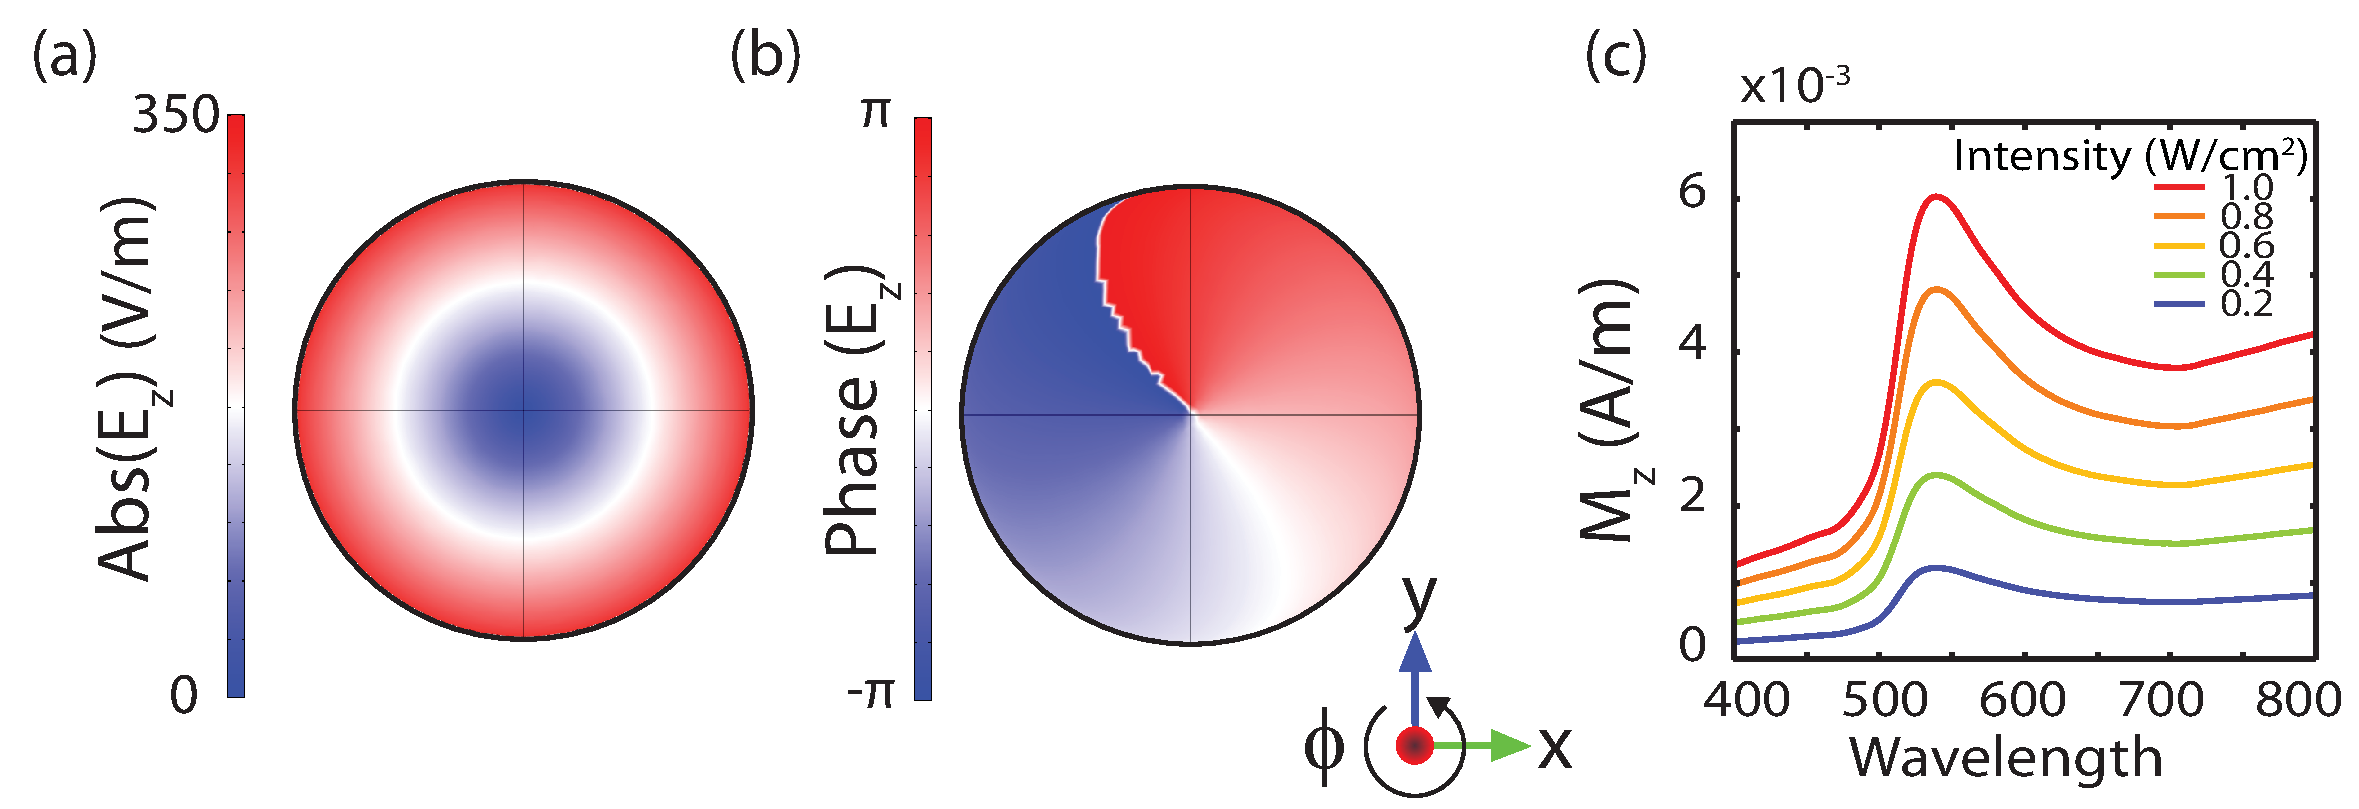
\includegraphics[width=0.95\textwidth]{EzMz}
\caption{Numerically calculated (a) amplitude and (b) phase of the longitudinal component of the electric field, $E_z$, with 540-nm 1 W/cm$^2$ RHCP illumination intensity. (c) Volume-averaged magnetization as a function of wavelength when illumination intensities are varied. All plots are for an aqueous 80-nm gold nanoparticle.}
\label{Ez}
\end{figure}

\subsection{Time-dependent response}
\indent The delayed optical response to an applied magnetic field is likely the result of the settling motion of non-spherical nanoparticles and nanoclusters. Aggregates often form as a result of random Brownian motion and magnetic-dipole interactions, so they are considered in this analysis. Also acknowledged are irregularities in the nanoparticles employed in the experiments-- they are not perfect spheres due to the fabrication process. Such variations from spherical geometry cause magnetization differences that depend on the nanoparticle orientation with respect to the electric field.
\\\indent Changes in extinction spectra reflect the magnetization associated with the nanoparticle and nanoclusters reorientation. Structural anisotropy and orientation affect the magnetization of the nanoparticle, which is illustrated with dimer nanoclusters and ellipsoids of different aspect ratios. As can be seen in Fig.~\ref{Dimer}(a) there is a reduction in the magnetization by almost 50\% as a dimer nanocluster rotates from minimal to maximal incident surface area with respect to electric field.
 The relative change in the magnetization is shown in Fig.~\ref{Dimer}(b) as a function of aspect ratio when ellipsoidal nanoparticles of equal volume are rotated from minimal to maximal incident surface area. Ellipsoids with aspect ratio 1 (spheres), exhibit no difference as they are rotated, and greater differences are observed when the aspect ratio increases. To guide the eye, a trendline that reflects the Biot-Savart law is provided in Fig.~\ref{Dimer}(b). Deviations from the trendline are attributed to changes in the plasmonic eigenfrequency. Regardless, anisotropy in the nanoparticle shape leads to MO magnetization that varies with the orientation, a concept in agreement with prior work~\cite{Jain,Funston}. 
\\\indent %Numerical simulations of dimer nanoclusters and ellipsoids indicate that structural anisotropy lead experimentally to torque forces that maximise MO and mechanical effects.
There exists a nanoparticle/nanocluster orientation with respect to the external magnetic field that maximises $\langle\vec{j_m}\rangle$. 
\begin{figure}[t]
\centering
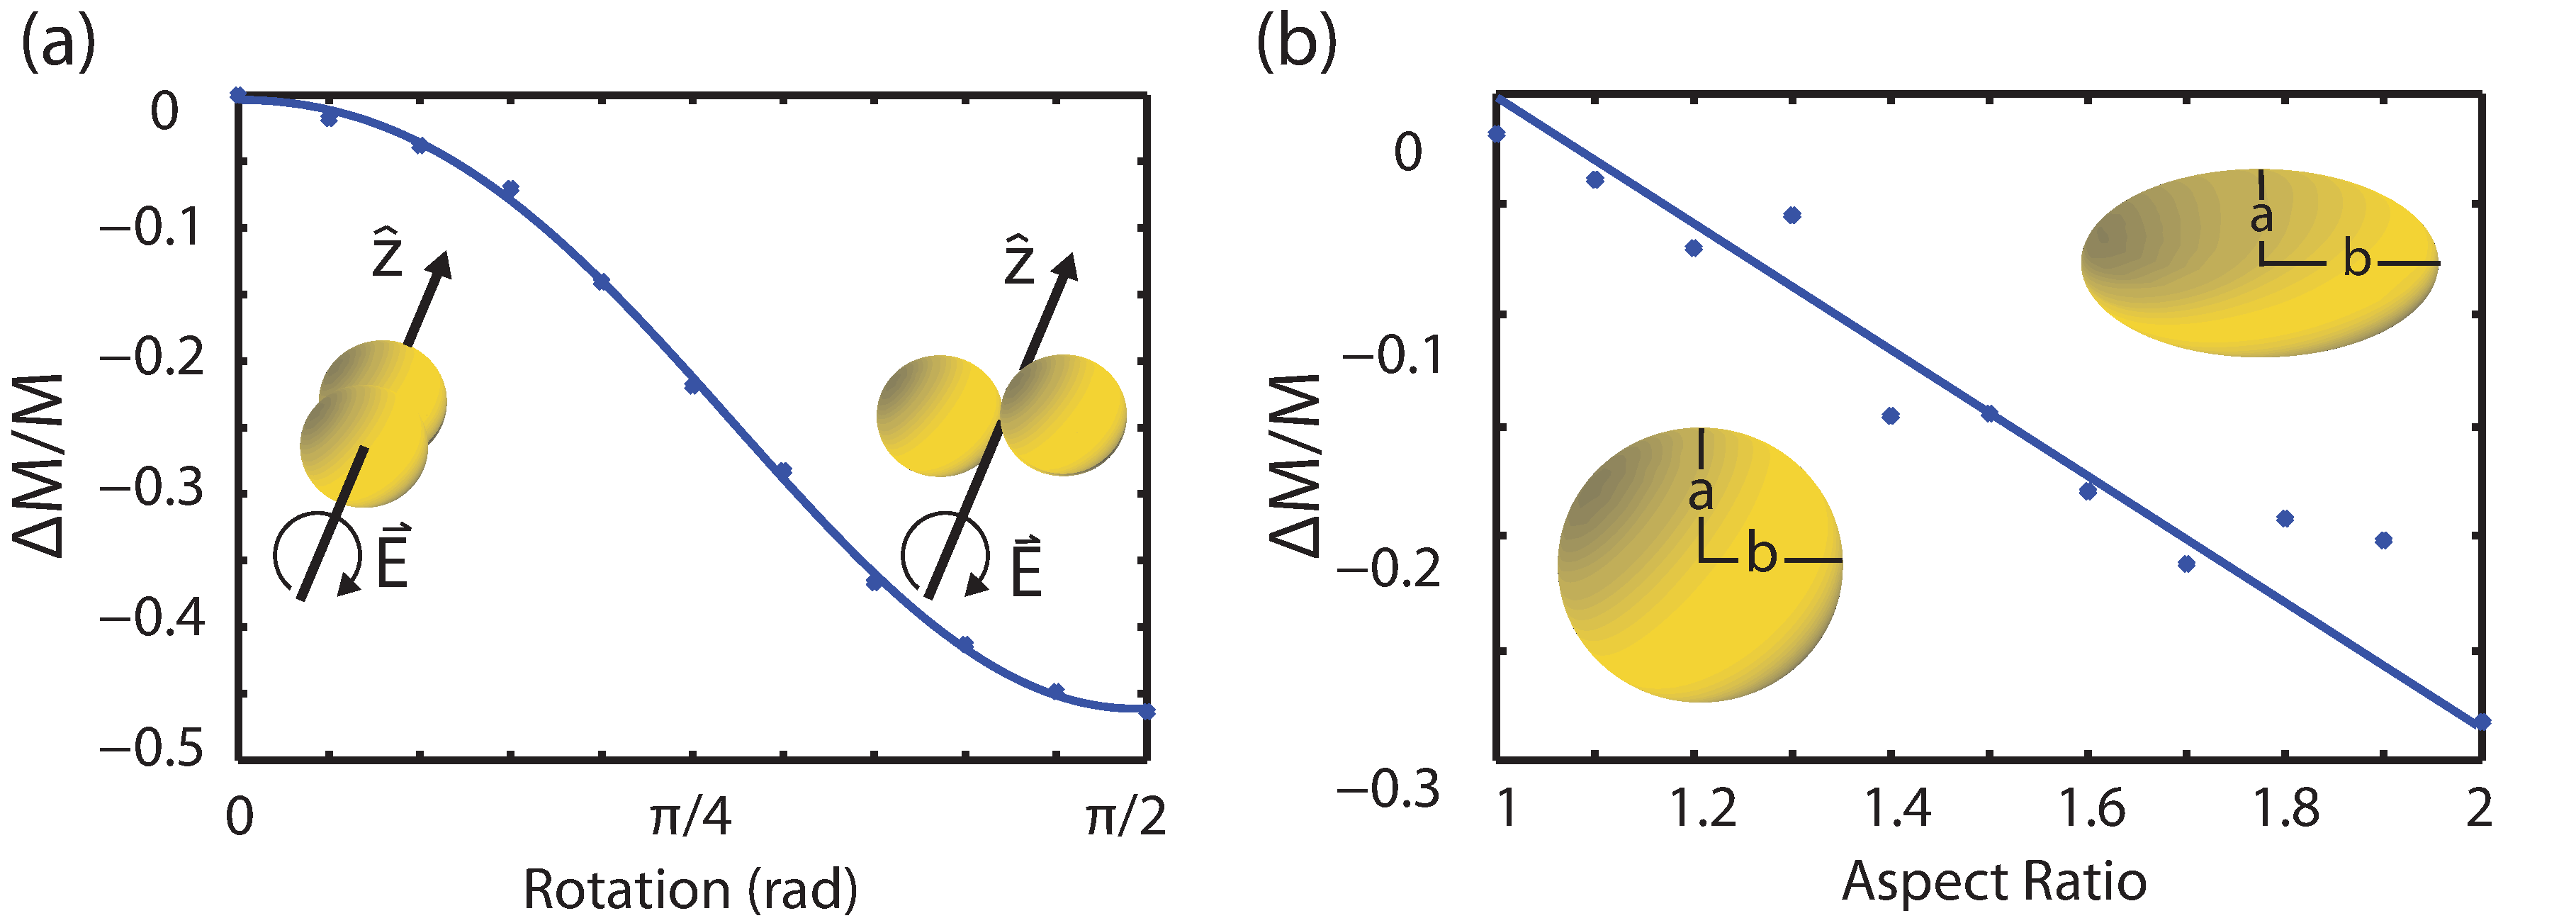
\includegraphics[width=0.95\textwidth]{MagPlots}
\caption{Numerically calculated relative change in magnetization (a) of a 80-nm gold dimer nanocluster as a function of angle of rotation, and (b) ellipsoidal gold nanoparticle rotated from minimal to maximal surface area as a function of aspect ratio, illuminated with 540-nm 1 W/cm$^2$ RHCP.}
\label{Dimer}
\end{figure}
The system is expected to stabilize in an orientation that maximises the nanoparticle magnetization. The nanocolloid magnetization is largest at the plasmon resonance when the local electric field and scattering is maximised.
\\\indent Yet, scattering dynamics present a complex dynamical system that is not fully understood in the context of MO responses. Autocorrelation data reveals significant pulse broadening through gold nanocolloid solution that scales with the square of the sample thickness that suggests a strong scattering [\cite{Genack}] despite low fill factors (2.5$\times 10^{-6}$). 
%The scattering cross-sections of metal nanocolloids are much greater than their geometrical cross-section at resonance~\cite{Mie}, and 5 orders than the light emission from strongly fluorescing dyes~\cite{Jain2}, indicating a strongly scattering medium. %Autocorrelation data shows significant pulse broadening through 400 $\mu$m of nanocolloid solution from 2.3 ps to 3.2 ps, which suggest appreciable multiple scattering events, despite low fill factors (2.5$\times 10^{-6}$). 
Another possibility for the larger-than-expected results is diffractive coupling between nanoparticles that can exhibit strong long-range interaction [\cite{Barnes2}] that lead to near-field enhancements, which are anticipated to increase in a 3-D matrix. The material properties of the matrix also influence the MO response. For instance, the presence of any ions or charged particles, common in solvents such as water, modifies the electrodynamics of the system, which subsequently influences the MO response of the system.
\section{Conclusion}
\indent This chapter demonstrates the observation of MO responses in non-magnetic nanocolloids at ultra-low illumination intensities and magnetic fields. Metal nanocolloids are magnetized and the optical properties are shifted when excited by coincident elliptically-polarized electric fields and DC magnetic fields. Experimentally-observed extinction spectra are in good agreement with predictions of linear and nonlinear MO effects and new considerations are provided for novel mechanical effects that were previously considered unattainable. A theoretical model is demonstrated that successfully explains the transition between linear and nonlinear MO plasmon dynamics of metal nanoparticles. This chapter provides the theoretical framework to study MO responses in non-magnetic nanostructures. In particular, new methods to identify, optically self-assemble and magnetically torque large quantities of disperse, non-spherical nanoparticles with broadband light sources are realised.

\section{Experimental difficulties and future work}
The experimental procedure to study the transmission properties were quite difficult. One recurrent issue that occurred was a time dependence in the transmission properties before any magnetic field was applied. This issue was attributed to thermal stabilization of the system and was overcome by waiting for the transmission properties to thermally stabilize before turning on the magnetic field and taking any measurements.

Care was also taken in the amount of light intensity, as it was found that if the light intensity was too great, there would be aggregation and settling of the nanoparticles at the bottom of the substrate. Aggregation may affect the results by shifting the plasmonic resonance of the nanoparticles due to the increase in size, which may confound the results. Settling of the nanoparticles is also undesirable since there is a reduction of the nanoparticle density interacting with the electric and magnetic fields that way decrease the MO effect and increase the transmission through the sample, confounding the results.

Future work on this subject may involve a deeper investigation of the threshold between the linear and nonlinear components that cause the respective transmission properties.